
\chapter{Search by Collage}
\label{ch:object_location}

% \todo[inline]{v grafe, na x ovu os dat rank}
% \todo[inline]{\% of searched target images up to a given rank}

\normalem
\emph{You see a picture in your head. Your friend is standing on the beach, and there is a little sandcastle on the left. The sea behind beautifully reflects the sun, which is setting.}
\ULforem

We can imagine that at that particular moment we were shooting a video of the scenery. However, years later, with a vast set of videos in our collections, it may be impossible to re-watch every one of them to find that particular memory. Not all of us can visualize the memory, but about those who can, we say that they have an excellent visual memory \footnote{\url{https://en.wikipedia.org/wiki/Visual_memory}}. We present a technique that can be used to search in a dataset based on such memories of the scenery.

In this chapter, we elaborate approaches for \acrlong{kis} based on a visual description of the memorized image. We characterise the image by the set of interesting objects in it, the way how they looked (by providing example images) and by their relative location in the image (i.e., top left corner). With that information, we look for a match in the database to the described image. We refer to our input as \emph{collage query}, or simply just as a collage. Collage is created by taking images and placing them onto an empty canvas. The placement of the images also carries a piece of information. We show an example of such a collage (query) in figure \ref{fig:query_collage_comparison}. On the left, we can see a cat in the center behind a window. On the right, we can see a possible visualization of such memory. On the grey canvas, we placed a window, which reminded us of the original one. At the center, we added a similarly colored cat.

\begin{figure}
\centering

\begin{subfigure}[t]{0.48\textwidth}
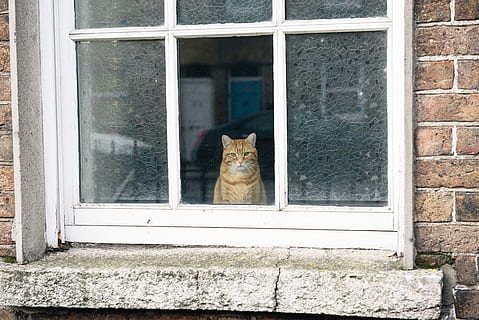
\includegraphics[width=0.95\linewidth]{img/cat_on_window} 
\caption{Target image}
\label{fig:searched_scene}
\end{subfigure}
\begin{subfigure}[t]{0.48\textwidth}
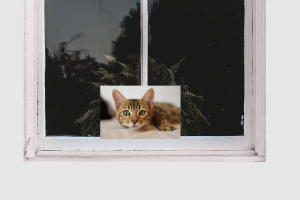
\includegraphics[width=0.95\linewidth]{img/cat_on_window_collage}
\caption{One of the possible collage descriptions of the target image}
\label{fig:collage_example}
\end{subfigure}

\caption{Example of searched image (target) with possible visual description by a collage.}
\label{fig:query_collage_comparison}
\end{figure}

While we were describing the image, we used words for it. However, in this chapter, we do not focus on the search based on the verbal description of the objects. Compared to such a textual approach, we can capture more diversity in the objects by visual information. For example, a single word for a human may represent a visually wide range of possibilities based on clothes, age and other attributes. These attributes are easier to capture by providing an example image. We can still struggle to find a similar image, that is why allowing collages is important. It is easier to put together several images together, each capturing some of the attributes, than finding an exact match.

This chapter presents three approaches incorporating pre-trained neural networks. We start with the formalization of the task. Next, we provide a short description of user-program interaction. Following the user interaction, we provide an overview of the framework and describe individual stages. Each of the stages is then separately discussed. 

After the discussion of the options for our system, we evaluate the proposed techniques. We firstly present a set of annotated data -- collages for the target images. Using these queries, we test different sets of hyperparameters and investigate their effect on the system's performance. 

\section{Formal description}
\label{s:task_formulation}

In this task, we explore the dataset $D$ based on a collage query provided by a user. We shall formally define universe of query images as follows: 
$$
    \mathcal{Q} = \{(I, x_0, x_1, y_0, y_1) | I \in \mathcal{U}, x_0 \in [0,1), y_0 \in [0, 1), x_1 \in (x_0, 1], y_1 \in (y_0, 1] \}
$$
where $\mathcal{U}$ is a universe defined in section \ref{s:task_formulation_preliminaries}. $I$ represents an image in the collage; $x_0$, $y_0$ represent the relative position of the top left corner of the image in the canvas; $x_1$, $y_1$ represent the relative position of the bottom right corner of the image in the canvas. Single collage $Q$ is then defined as $Q \subset \mathcal{Q}$

Ultimately, we would like to construct a function $r^*$, that for each query $Q_i \subset \mathcal{Q}$ would find corresponding target image $t_i \in D$. Formally, we can define this function as follows:
$$
    r^*: \mathcal{P(Q)} \rightarrow D 
$$
$$
    r^*(Q_i) = t_i \,\,\, \forall (Q_i, t_i) \in X
$$
where $X$ is a set of target images and corresponding queries constructed by the user.

However, due to imperfect user queries, or by the fact that user can search two different target images using the same collage, this task may be even impossible. Therefore, we focus on reordering the dataset in the way that linear search by the user in this order would provide the target image as quickly as possible. We define \emph{ranking} $r_{D}$ as function with respect to a given dataset $D$:
$$
    r_D: (D \times \mathcal{P(Q)}) \rightarrow \{0, 1, \ldots, |D|-1  \}
$$
$$
    \text{ s.t. } \{r_D(d, Q) \mid d \in D \} = \{0, 1, \ldots, |D|-1  \} \,\, \forall Q \subset \mathcal{Q}
$$

% TODO, je to function a for fixed Q je to ranking

For example, $r_D(t, Q) = n$ means that target image $t$ is at position $n$ after ordering the dataset $D$ with respect to collage $Q$. This value correlates with the time spent on the linear search of the provided ordered results. This gives us the motivation to evaluate our algorithm based on this \emph{rank} across the whole set $X$.

In our approaches, we construct such ranking based on the appropriate dissimilarity score $\delta': (\mathcal{U} \times \mathcal{P(Q)}) \rightarrow \mathbb{R}$. We discuss various choices of the dissimilarity score function further in the chapter. Then we may define the ranking as:
$$
    r_D(d, Q) = \abs{\{d' \in D : \delta'(d', Q) < \delta'(d, Q)\}}
$$

% Note that we do not compare the images directly, rather their descriptors, i.e.:
% $$
%     \delta'(x, y) = \delta(f_e(x), f_e(y))
% $$

However, such construction may break the requirements on the ordering. Therefore, we need to ``break ties'', we do so in arbitrary fashion:
$$
    r_D(d, Q) = \abs{\left\{d' \in D : \delta'(d', Q) < \delta'(d, Q) \lor \left(\delta'(d', Q) = \delta'(d, Q) \land d' <_a d\right)\right\}}
$$
where $<_a$ is any arbitrary total ordering of the dataset $D$. For theoretical purposes we could use the lexicographical ordering. In the implementation, we make use of a priori ordering of the dataset $D$ for this as ordering $<_a$.

\section{User-program interaction}

We provide the user with a canvas where they can place, move, and resize the collage images. They can add images by providing an URL of the image, or by pasting the image from a clipboard. One possible way to obtain images for the collage is to use an image search engine (e.g., Google Images). The images can be usually copied to the clipboard by selecting copy in the right-click menu. A quicker approach, we preferred, is using selective screenshots. With the selective screenshot, we can even crop the image, focusing on the part we like, and paste it onto the canvas.

Based on the provided collage, the program searches for similar images in the dataset and interactively presents them back to the user. The user can then alter the query for a new search, or investigate the displayed results. Figure \ref{fig:collage_example} shows an example of the query -- the collage of two images (window and cat). 

\section{Framework overview}

\begin{figure}[p!]
    \centering
    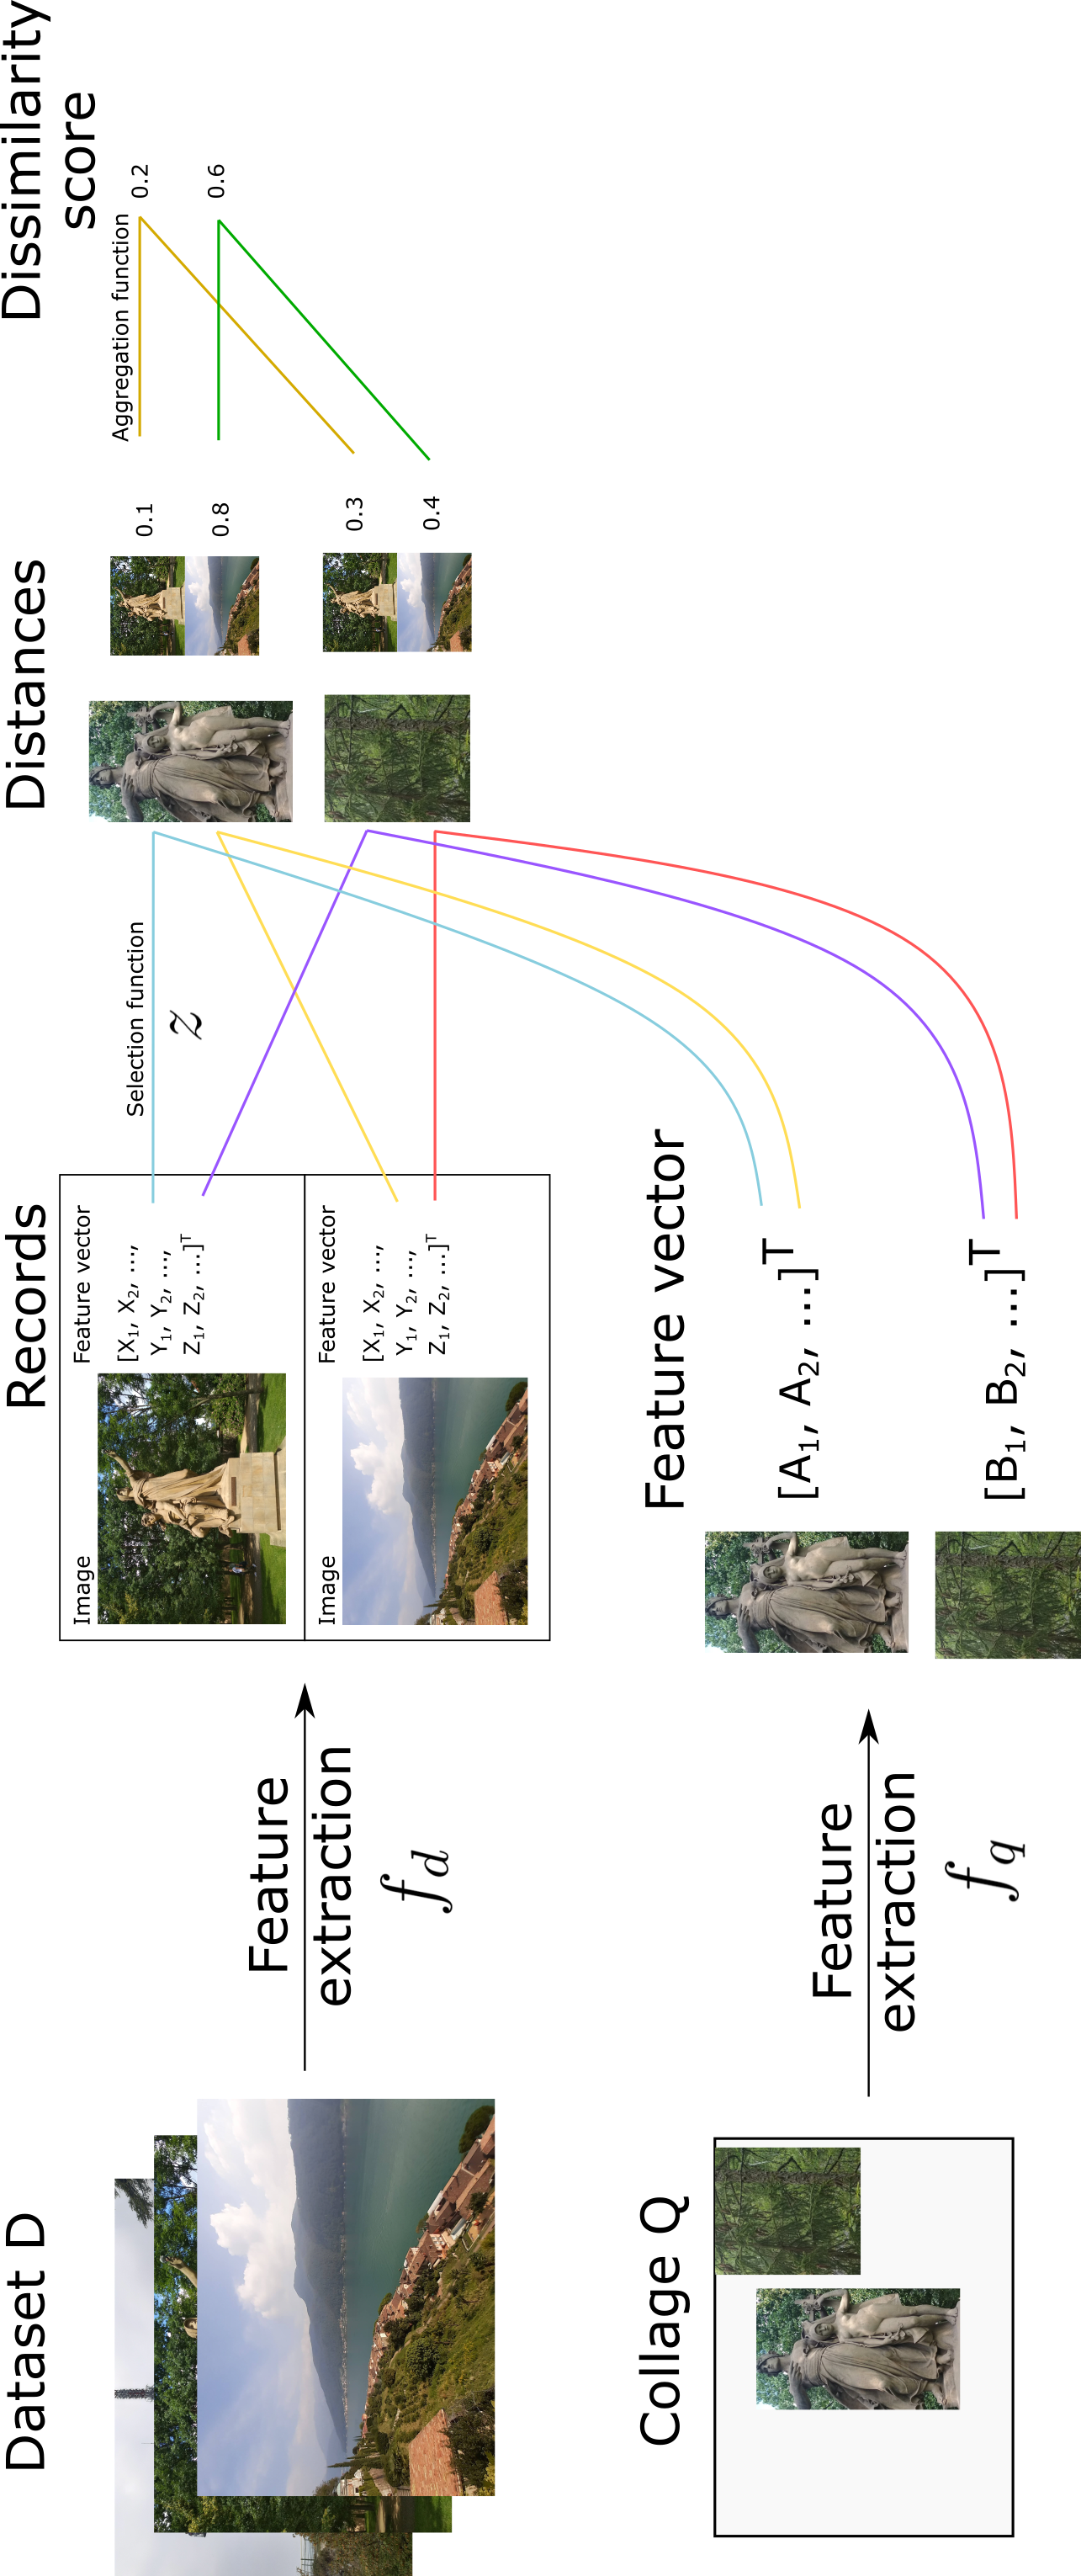
\includegraphics[scale=0.9]{img/features_pipeline.png}
    \caption{Overview of processing pipeline}
    \label{fig:processing_pipeline}
\end{figure}

Our approach consists of several individual steps. Figure \ref{fig:processing_pipeline} shows a visual overview of the steps we describe here. Our first step is to compute feature vector for each image, given the descriptor extraction function. We call this step \emph{feature extraction}. This way, we obtain records, i.e., a pair of image from the dataset and its corresponding feature vector. We denote this feature extraction function as $f_d:\mathcal{U} \rightarrow \mathbb{R}^k$.

We often split feature vector into several parts (each describing only a part of the image). Appropriate part is then selected based on the position of the query image in the canvas and compared with the descriptor of the collage image. We denote \emph{selection function} $z: (\mathbb{R}^k, [0,1]^4) \rightarrow \mathbb{R}^n$, where $[0,1]^4$ refers to the position of the image in the canvas.

In the collage processing path, we use feature extraction function $f_q: \mathcal{U} \rightarrow \mathbb{R}^n$ to obtain feature vectors of the images from the query collage (one vector for each image). This part is done online; therefore, we need to obtain the descriptors on the fly to perform the search. Since we only extract descriptors for a couple of images, it is possible to use the predictions from the neural networks even without the access to GPU.

As the next step, our goal is to obtain the distance for descriptor of each query image and descriptor of each image in the dataset, i.e., between the results of $f_q$ and $z$. Finally, we obtain for each image in the dataset a multiset of distances. We \emph{aggregate} these distances in order to compute the final dissimilarity score. Based on the dissimilarity scores, we compute the final \emph{ranking}, as described in section \ref{s:task_formulation}.

To summarize, we compute the dissimilarity score $\delta'(d, Q)$ between $d \in D$ and collage $Q \subset \mathcal{Q}$, we do following:
$$
   \delta'(d, Q) = A(\{\delta(f_q(q_u), z(f_d(d), q_m)) \mid q\in Q\})
$$
where $A$ denotes the aggregation function over a multiset. We use notation $q = (q_u, q_m)$, where $q_u$ represents the collage image and $q_m$ the metadata, i.e., position in the canvas. Also, in this particular equation, we use the $\{(\cdot)\}$ for a multiset.

While the described pipeline offers a reasonably straightforward approach to the task at hand, the individual stages' internal factors require a fair amount of tuning. We evaluate the hyperparameters with respect to the performance of the whole framework. Throughout the following sections, we progressively build the pipeline while describing the particular approaches we use. We start with the discussion on feature extraction, and then progress towards the next stages of the system.  

\section{Features extraction strategies}

In the following section, we present three feature extraction techniques. We begin this section with the description of the baseline model. The baseline model does not use the spatial information about the images in the collage. This baseline approach is currently used, for example, by the VIRET tool \citep{kovalvcik2020viret}. 

Following the baseline model, we present two approaches which utilize the spatial information from the collage. The first one splits the images in the dataset to fixed regions. The second one utilizes information from the neural network before the last pooling layer.

\subsection{Baseline -- Image representation}

The baseline ignores the spatial information of the images in the collage. We set this approach as our baseline since it is relatively simple and can solve our task. In this baseline approach, we compute the feature vector for an image in the dataset using a deep neural network as a descriptor extraction function, and directly compare them with the descriptors of the collage's images.

In this approach we use a given \acrshort{cnn} to obtain the descriptors of the collage's images and also dataset images. Therefore, $f_q = f_d$. Since, we directly compare the descriptors, the selection function $z(x, q_m) = x$.

Since the resolution of the query images and images in the dataset may not match the input shape of the \acrshort{cnn}, we rescale them to the required input size.

\begin{figure}
\centering
\begin{boxedverbatim}
Dataset:
    - image: 1 feature vector
Query:
    - query_image: 1 feature vector
    - compared to: each feature vector in the dataset
\end{boxedverbatim}
\caption{Overview of the Baseline -- Image representation approach}
\end{figure}

\subsection{Splitting the image into regions}

In the next presented approach, we will focus on using the spatial information of the images in the collage. This position of the objects can serve as highly distinguishing criteria while looking for the target image. In the previous subsection, we described the image in the dataset by only one prediction of the neural network. We obtain higher granularity for the data, by splitting the image into multiple regions and then computing the feature vector on each of the region separately.

Let us assume that, we split the image into $m$ cuts. For each image of the dataset, we now need to store $m$ times more information. Resulting feature vector is of space $\mathbb{R}^{nm}$, where $n$ is the size of the \acrshort{dnn} output. To avoid increasing the time complexity by the multiplicative factor of $m$, we investigate a principle, how to compare the query image only with the one or few out of these $m$ cuts and not to all. That way, we preserve the same time complexity except for some additive factor, compared to the Baseline.

First we describe the selection of the cuts, and then we discuss the principle of selection for the cuts. The overview of the information preserved for this approach is in figure \ref{fig:overview_regions}.

\begin{figure}
\centering
\begin{boxedverbatim}
Database:
    - image:
        - multiple crops:
            - crop's position
            - feature vector
Query:
    - query_image: 1 feature vector
    - compared to: only to selected crops from each image
\end{boxedverbatim}
\caption{Overview of the regions' approach}
\label{fig:overview_regions}
\end{figure}

\subsubsection{Cutting the image}

Each image in the dataset is divided into $N \times M$ regions. Descriptor is then computed and stored for each region separately. The defined cutting is identical for all images in the dataset.

First, we discuss the choice of the shape of the regions into which we want to split the images. Since we plan on feeding the region's image into a CNN, we set a limitation on using only square regions. This limitation comes from the fact that common CNN architecture expects a square image on the input. We could, in theory, rescale rectangular regions into squares, but this would induce a non-necessary distortion of the image. We avoid this distortion by posing this simple condition on the regions' shape.

We test several sizes of the input squares in the experiments. Although, we limit ourselves to the input shapes, for which a pre-trained CNNs are available. This for example for MobileNetV2 includes the following shapes: $96 \times 96, 128 \times 128, 160 \times 160, 192 \times 192$ and $224 \times 224$.

We impose a second limitation on the choice of regions. We require that their union fully covers the input image. In that way, information from each part of the image is extracted. Also, we do not allow the regions to extend over the image. 

Our limitations summarized are square regions, not extending over the image and full coverage of the input image. Except for a particular case, when the width and height would be divisible by the input shape dimension, the regions must overlap. The special case does not arise in our dataset, as we work with images $320 \times 180$.

We propose a cutting, which for the desired number of regions $N \times M$ with the desired width $s$ of the region, produces evenly distributed regions. In case the regions cover greater area than the image itself (that is, $sN > h$, where $h$ is the height of the image), the regions are evenly distributed over the axis.

The side effect of the overlaps also plays an important role in this technique. With the rigid frame without overlapping, we could face a situation where a single object would be split into two separate parts. Both parts separately could lack enough visual information on the object to provide consistent results. With the excess distributed to all regions, we share the information alongside the cut to both regions.

Our fixed parameters are regions' width $s$ and the number of regions we want to use $N \times M$ and image size $h, w$. We solve the task of choosing regions splits for one axis; the second is done analogously. We know that the last region has to end with the edge of the image. Therefore, the starting coordinate of the last region is $h - s$. We then split the remaining ``space'' (space not covered by the last region) over $N-1$ regions equally. We call this distance $step$ since it says the distance between the starting points of the regions. The starting coordinate $r_i$ of the $i$-th region in a given axis is:

\begin{align*}
step_h = (h - s) / (N - 1) \\
r_i = {i \, step_h\,\,\text{for}\,i \in \{0, 1, 2, \dots, N - 1\}}
\end{align*}

With the condition on full coverage of the image (i.e., $s N \geq \text{h}$, and for $M$ respectively), we obtain full coverage of the image by the regions. Overlaps are evenly distributed over both axes. Note that, with bigger sized regions, overlaps may occur between more than two regions. For example, if we split an image with width 180 into three regions with a width of 96 pixels, some areas of the image will be included in all three regions. This happens when the $step < s/2$.

\subsubsection{Selecting regions}

Previously, we defined cutting into the regions for each item in the dataset. One of the possible steps further in the pipeline could be to compare all regions' feature vector to the query image feature vector. Although this would be an entirely valid approach, it has two caveats: firstly, it does not take advantage of knowing the position of the query image in the collage, and secondly, it multiplicatively increases the time required, when comparing to $N \cdot M$ more feature vectors, than before.

We discuss the options of selecting only relevant regions to the query image based on the position of the query image. Given one query image with its position and shape, we propose the following methods for choosing the relevant regions:
\begin{itemize}
  \item choosing only the one, which is covered the most by the query image,
  \item choosing all regions, which have a non-empty intersection with the query
  \item or approaches in between, by setting a maximum to a number of relevant regions.
\end{itemize}

We visualize the problem in figure \ref{fig:fish_with_grid}. The query would be an image of the fish placed as the red boundary shows. All regions with a nonempty intersection with the query image are highlighted in green. The region with the highest ``coverage'' is the blue one.

To make this idea over coverage measurable, we use the Jaccard index. We compute the Intersection over Union between the region and the crop, where the query image is located. 

\emph{Intersection over Union} (also known as Jaccard index\footnote{\href{https://en.wikipedia.org/wiki/Jaccard_index}{https://en.wikipedia.org/wiki/Jaccard\_index}}) measures similarity between two sets. We use it as a metric to express how much region and query image overlap. 

The definition of the Intersection over Union is following:
$$
    J(A, B) = 
    \begin{cases}
      1, & \text{if\ A and B are empty} \\
      \frac{|A \cap B|}{|A \cup B|}, & \text{otherwise}
    \end{cases}
$$

In our case, the $|A \cap B|$ represents the area that belongs to both, region and query image. The  $|A \cup B|$ represents the area covered by the union of both. A visual representation of the formula is displayed in the figure \ref{fig:intersection_over_union}. Using this index, we can order the regions based on their coverage with the query image. The more relevant regions are the ones with the higher Intersection Over Union with the query image and vice versa. Please note, that in our particular case, measuring the \acrshort{iou} leads to the same results, as considering only the size of the overlap. However this notation allows for future work to use regions of various sizes.

\begin{figure}
    \centering
	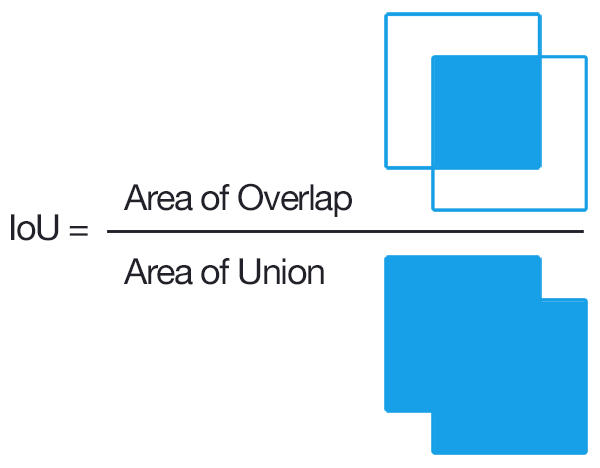
\includegraphics[width=0.4\linewidth]{img/Intersection_over_Union_-_visual_equation.png}
	\caption[Intersection over Union between regions]{Intersection over Union between regions. Source: Wikipedia, CC BY-SA 4.0}
	\label{fig:intersection_over_union}
\end{figure}

From the regions ordered by their \acrshort{iou} to the query image, we select the first $n$. We leave $n$ as one of our hyperparameters to evaluate in the experiments. Recall that the required output of this stage is only one descriptor, not multiple from multiple regions. Therefore, when we compare the feature vectors with multiple regions, we select only a winner, with the lowest distance for the next phase. 

\begin{figure}
\centering
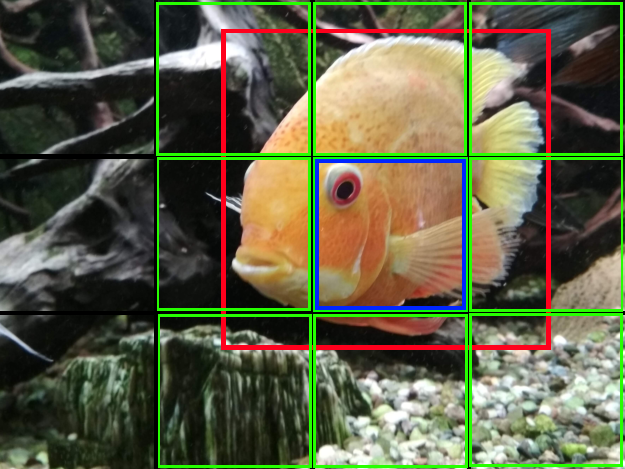
\includegraphics[width=0.63\textwidth]{img/fish_grid_regions}
\caption[Example of choosing the corresponding regions]{Example of choosing the corresponding regions. Red: query position; Green: all intercepted regions; Blue: region with highest IoU.}
\label{fig:fish_with_grid}
\end{figure}

\subsection{Using the representation before pooling}

The disadvantage of the previously presented technique is fixed cutting. The cutting into regions does not adapt to the size of collage image. 

Let us retake a look at the fish in figure \ref{fig:fish_with_grid}. We can see that fish covers approximately two-thirds of the image, but the individual regions cover only one-twelfth. In this case, only this one-twelfth of the image is compared to the query image. The method is missing any adaptation on the size of the query image.

After investigating the structure of the CNNs, we propose an approach based on the information obtained in the last convolution block. In standard architectures, after the last convolution block follows a pooling layer. So far, we only worked with the representation based on this pooling layer.

In this approach we work with the results before applying pooling. As we have stripped two layers from the classification \acrshort{cnn} -- the fully connected layer used for classification, and the pooling layer --, we also refer to this method as ``antepenultimate'' (meaning ``last, but two'').

Since the results we now work with are obtained before global pooling, i.e., from the last convolution block, they are from higher-dimensional space. The space of the feature vectors is now $\mathbb{R}^{k\times l \times c}$. Typically, this space is reduced to $\mathbb{R}^c$ by the global pooling layer.

Due to the way how CNNs work, we assume we could use the information about the query position, to work only with the part of the feature vector provided by the antepenultimate layer. The overview of the method is available in figure \ref{fig:antepenultimate_overview}

\begin{figure}
\centering
\begin{boxedverbatim}
Database:
    - image:
        - 1 feature vector (the result before pooling):
Query:
    - query_image: 1 feature vector after pooling
    - compared to: pooling over selected region
\end{boxedverbatim}
\caption{Overview of using the representation before pooling}
\label{fig:antepenultimate_overview}
\end{figure}


\subsubsection{Choosing a region of interest in the layer}

Layer before pooling on which we focus (antepenultimate) is the last convolution block. Therefore, it produces features from space $\mathbb{R}^{K\times L \times C}$, where $K, L, C$ is the shape of the convolution block output. The first two dimensions represent the spatial information, which is propagated from the previous layers. The third represents the channels (i.e., features).

To obtain only the part of this layer we are interested in (i.e., our query was placed in that specific region), we need to take only a subset over the first two dimensions. For a query $Q_i = (I, x_0, y_0, x_1, y_1)$ and a hidden layer $L_i$ represented as a matrix $K \times L \times C$ we select a submatrix based on the query position. 

Let the $rows$ and $cols$ be the indexes of the selected rows and columns, respectively. 
$$
    rows =
    \begin{cases}
        \{\nint{y_0 K}, \nint{y_0 K} + 1, \ldots, \nint{y_1 K}-1\} & \text{if } \nint{y_0K} < \nint{y_1K} \leq K \\
        \{\nint{y_0K}\} & \text{if } \nint{y_0K} = \nint{y_1K} < K\\
        \{K-1\} & \text{if } \nint{y_0K} = \nint{y_1K} = K\\
    \end{cases}
$$

$$
    cols =
    \begin{cases}
        \{\nint{x_0 L}, \nint{x_0 L} + 1, \ldots, \nint{x_1 L}-1\} & \text{if } \nint{x_0L} < \nint{x_1L} \leq L \\
        \{\nint{x_0L}\} & \text{if } \nint{x_0L} = \nint{x_1L} < L\\
        \{L-1\} & \text{if } \nint{x_0L} = \nint{x_1L} = L\\
    \end{cases}
$$

where the $\nint{(\cdot)}$ represents rounding to the nearest integer. We then select the submatrix $L_i'$ of the $L_i$ as: 
$$
L_i' = L_i[rows; cols; \{0, 1, \ldots |C|\}]
$$

Both MobileNetV2 and Resnet50V2 end with a convolution block with dimensions $(7,7,C)$, where $C = 1280$ for MobileNetV2 and $C = 2048$ for Resnet50V2. 

In this phase, we have selected a submatrix $L_i'$ with respect to the position of the query image. We apply global average pooling, as was applied in the original network over the layer $L_i'$. 

Performing the global average pooling over a given matrix $A$ with the dimensions $K' \times L' \times C$ produces vector $(b_0, b_1, \ldots, b_{C-1}) \in \mathbb{R}^{C}$:
$$
    b_i = \frac{\sum_{k=0}^{K'-1} \sum_{l=0}^{L'-1} a_{k, l, i}} {K'L'} \,\, \forall i \in \{0, 1, \ldots C-1\}
$$

where $a_{k,l,i}$ represents an element of the $A$ in $k$-th row, $l$-th column and $i$-th channel.

Finally, by performing the global average pooling over $L_i'$, we obtain our feature vector, which is later used.

Compared to the previous approaches, we aimed to avoid the strict cutting and to provide more flexibility. The caveat of this approach is increased memory consumption, since we store 49 feature vectors per vector ($7\times7$). It also requires to compute the average pool for each of the query images separately. Therefore, the time complexity is also increased. The factor is multiplicative, by the number of images in the collage and the size of the used layer.

\section{Ranking}

Let us remind an overview from figure \ref{fig:processing_pipeline}. In the previous section, we have seen three approaches presented for feature extraction and the extraction of the relevant features. The first presented approach is the baseline; the second cuts the image into regions and the third uses information from the antepenultimate layer of CNN. Now we shall focus on the remaining steps in the pipeline.

The first of these steps is computing distance between the descriptors of collage images and descriptors of dataset images. We  evaluate all distance function mentioned in the section \ref{s:distance_measures}.

Then we proceed to compute the dissimilarity score between the collages and images in the dataset. We do so by aggregating computed distances by the aggregation function $A$. Again, we test and evaluate various aggregation functions: minimum, maximum, and average.

As the final step, we compute the ranking, as defined in section \ref{s:task_formulation} using computed dissimilarity scores.

\section{Additional parameters}

In addition to different techniques of obtaining the feature vectors, we also inspect several other parameters of the system. These parameters include pre-processing of the collage images, post-processing of the features, and selecting the specific \acrshort{cnn}. This section further discusses these parameters.

\subsection{Padding}

We talked about the importance of the square input in the regions section. Although, so far, we did not discuss how we handle the case when the user provides a non-square image to the collage.

The option to create non-square queries comes handy when the user wants to include, for example, a picture of a standing person, or a kayak. A question arises, what is the best way to edit the image before feeding it to CNN. We test three techniques: rescale, black padding, and white padding. Example of applying these techniques on an image is shown in figure \ref{fig:penguin}. We have previously discussed the caveats of the rescale -- it distorts the images. If the person in the query image is in a tall and narrow box, the distortion will cause it to appear more full and shorter. The distortion becomes stronger with an increasing imbalance between the box dimensions. The alternative approaches, black and white padding, differ only in the filling color. The padding works by adding stripes of the given color to make the originally shorter side the same length as the other. The stripes are of the same size, so the original image is centered along the axis that was shorter. 

\begin{figure}
     \centering
     \begin{subfigure}[b]{0.3\textwidth}
         \centering
         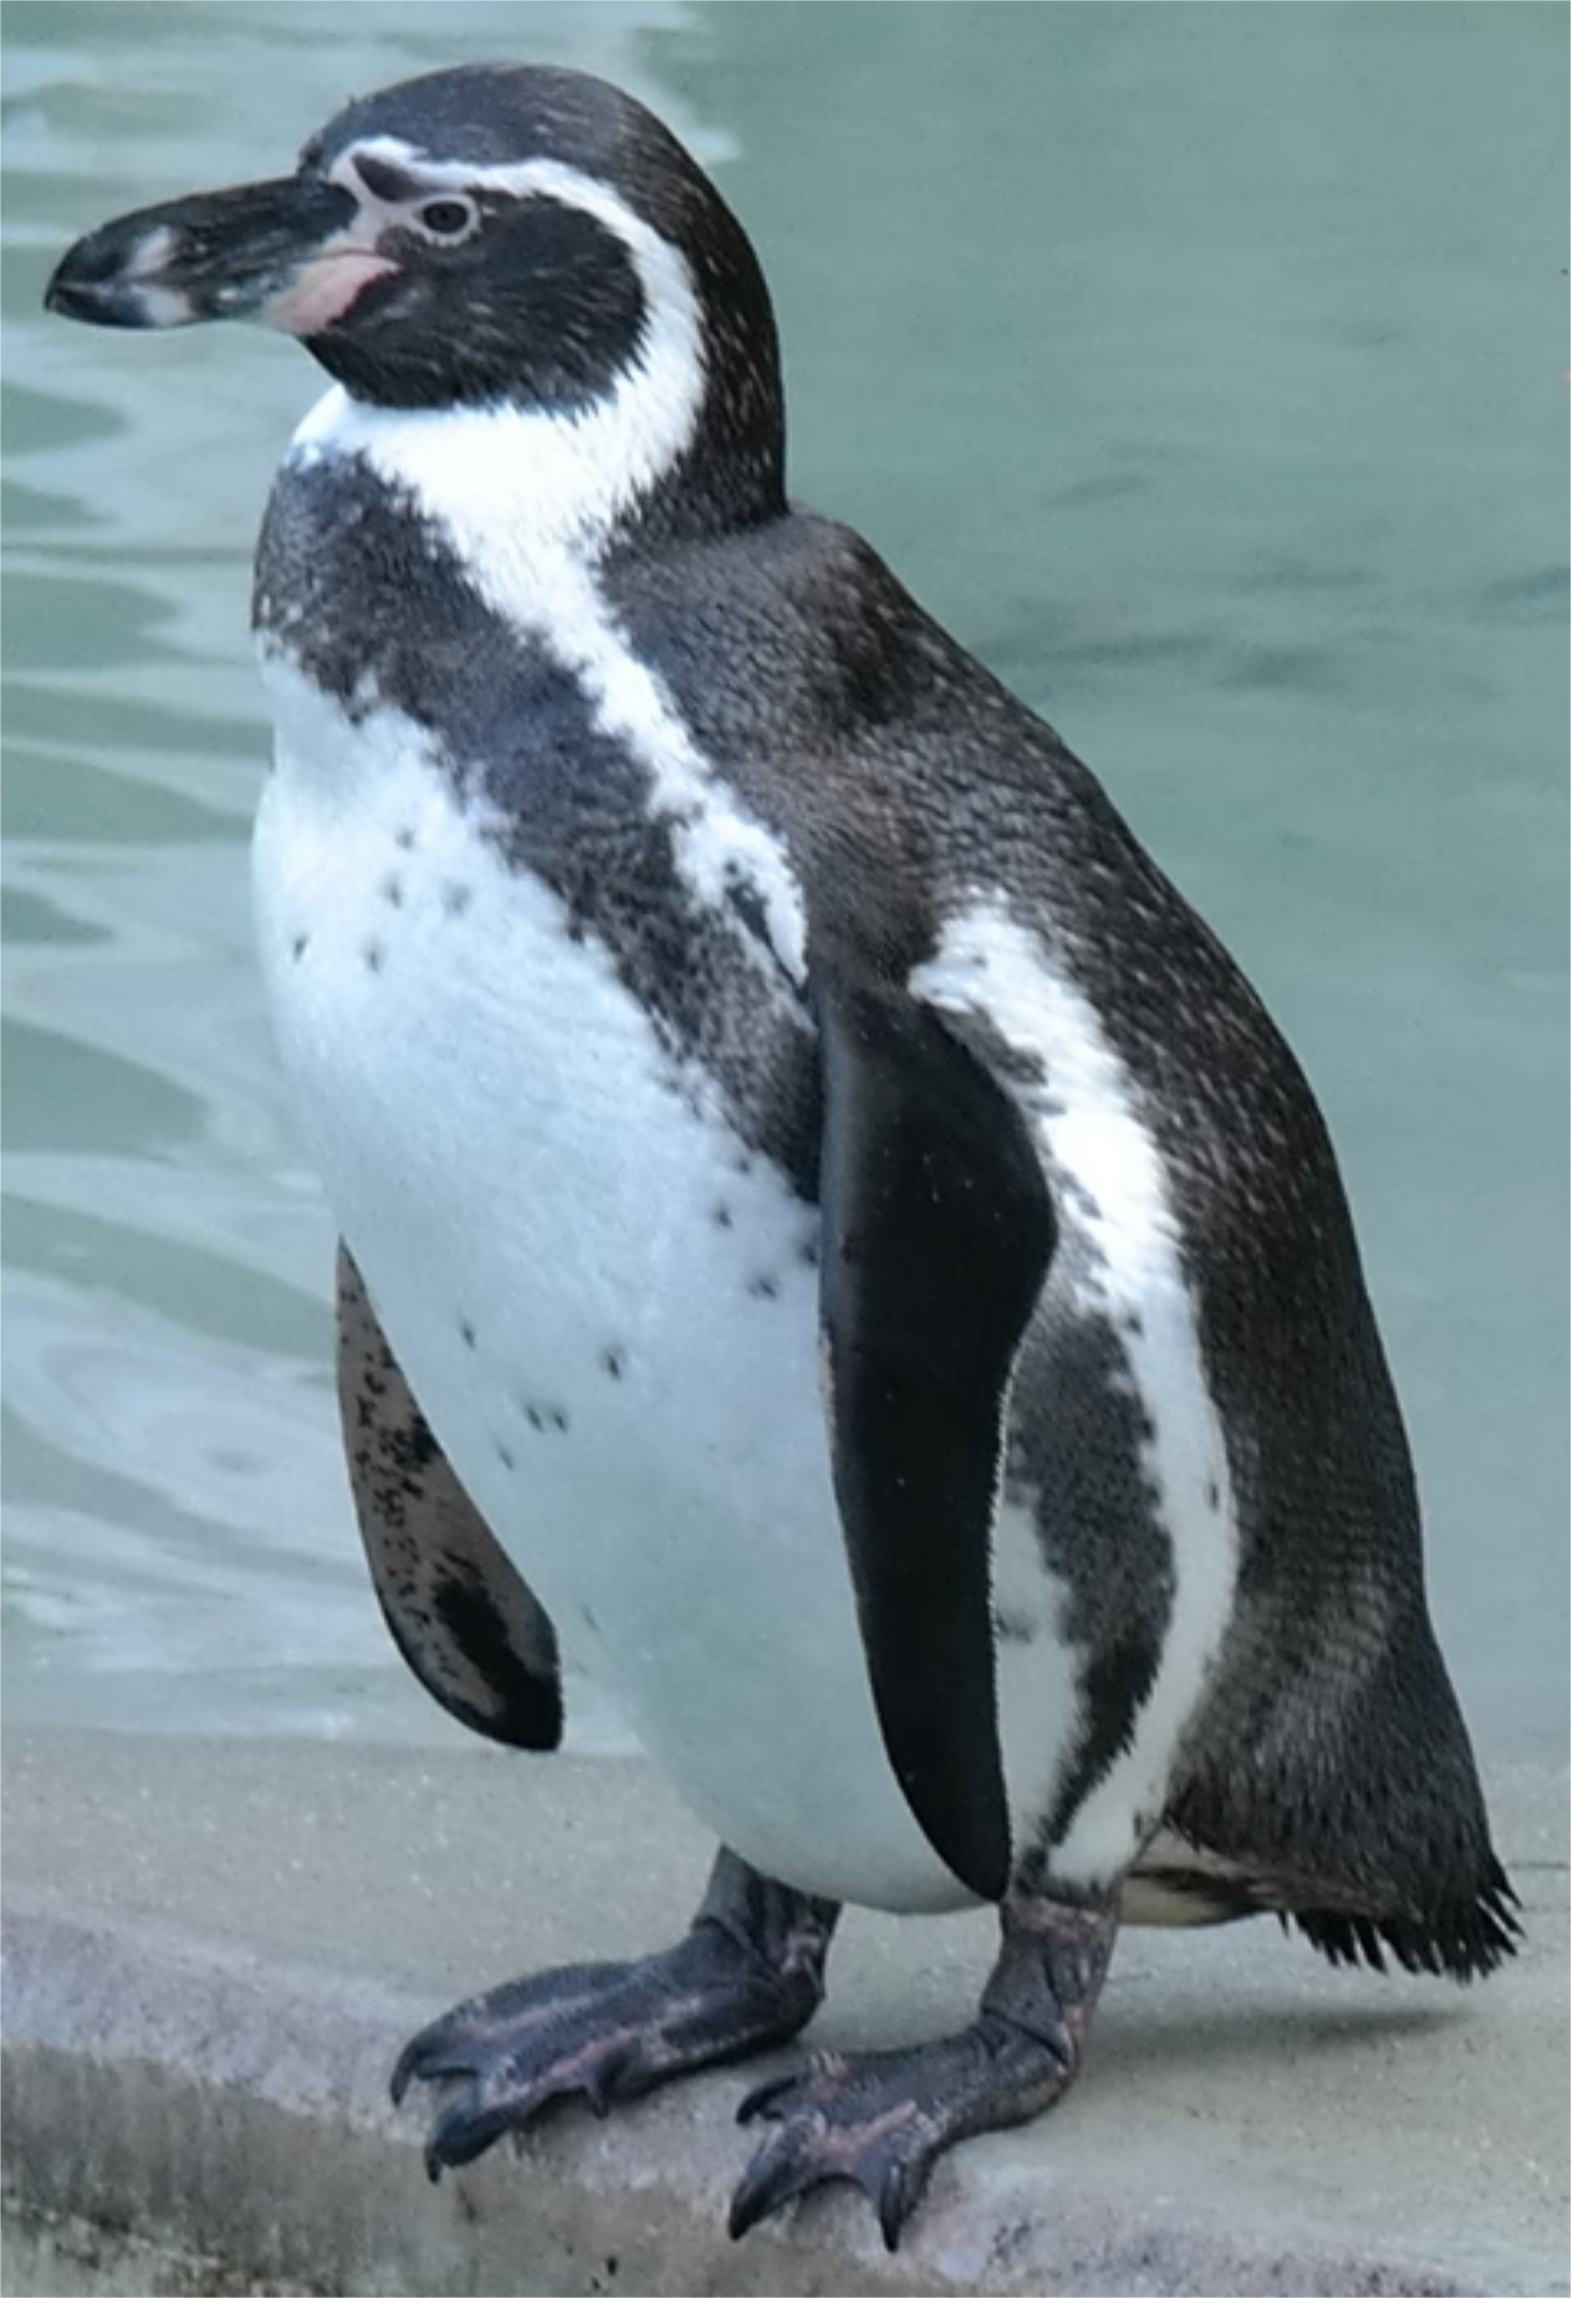
\includegraphics[height=4.2cm]{img/original.png}
         \caption{Original image}
     \end{subfigure}
     \hfill
     \begin{subfigure}[b]{0.3\textwidth}
         \centering
         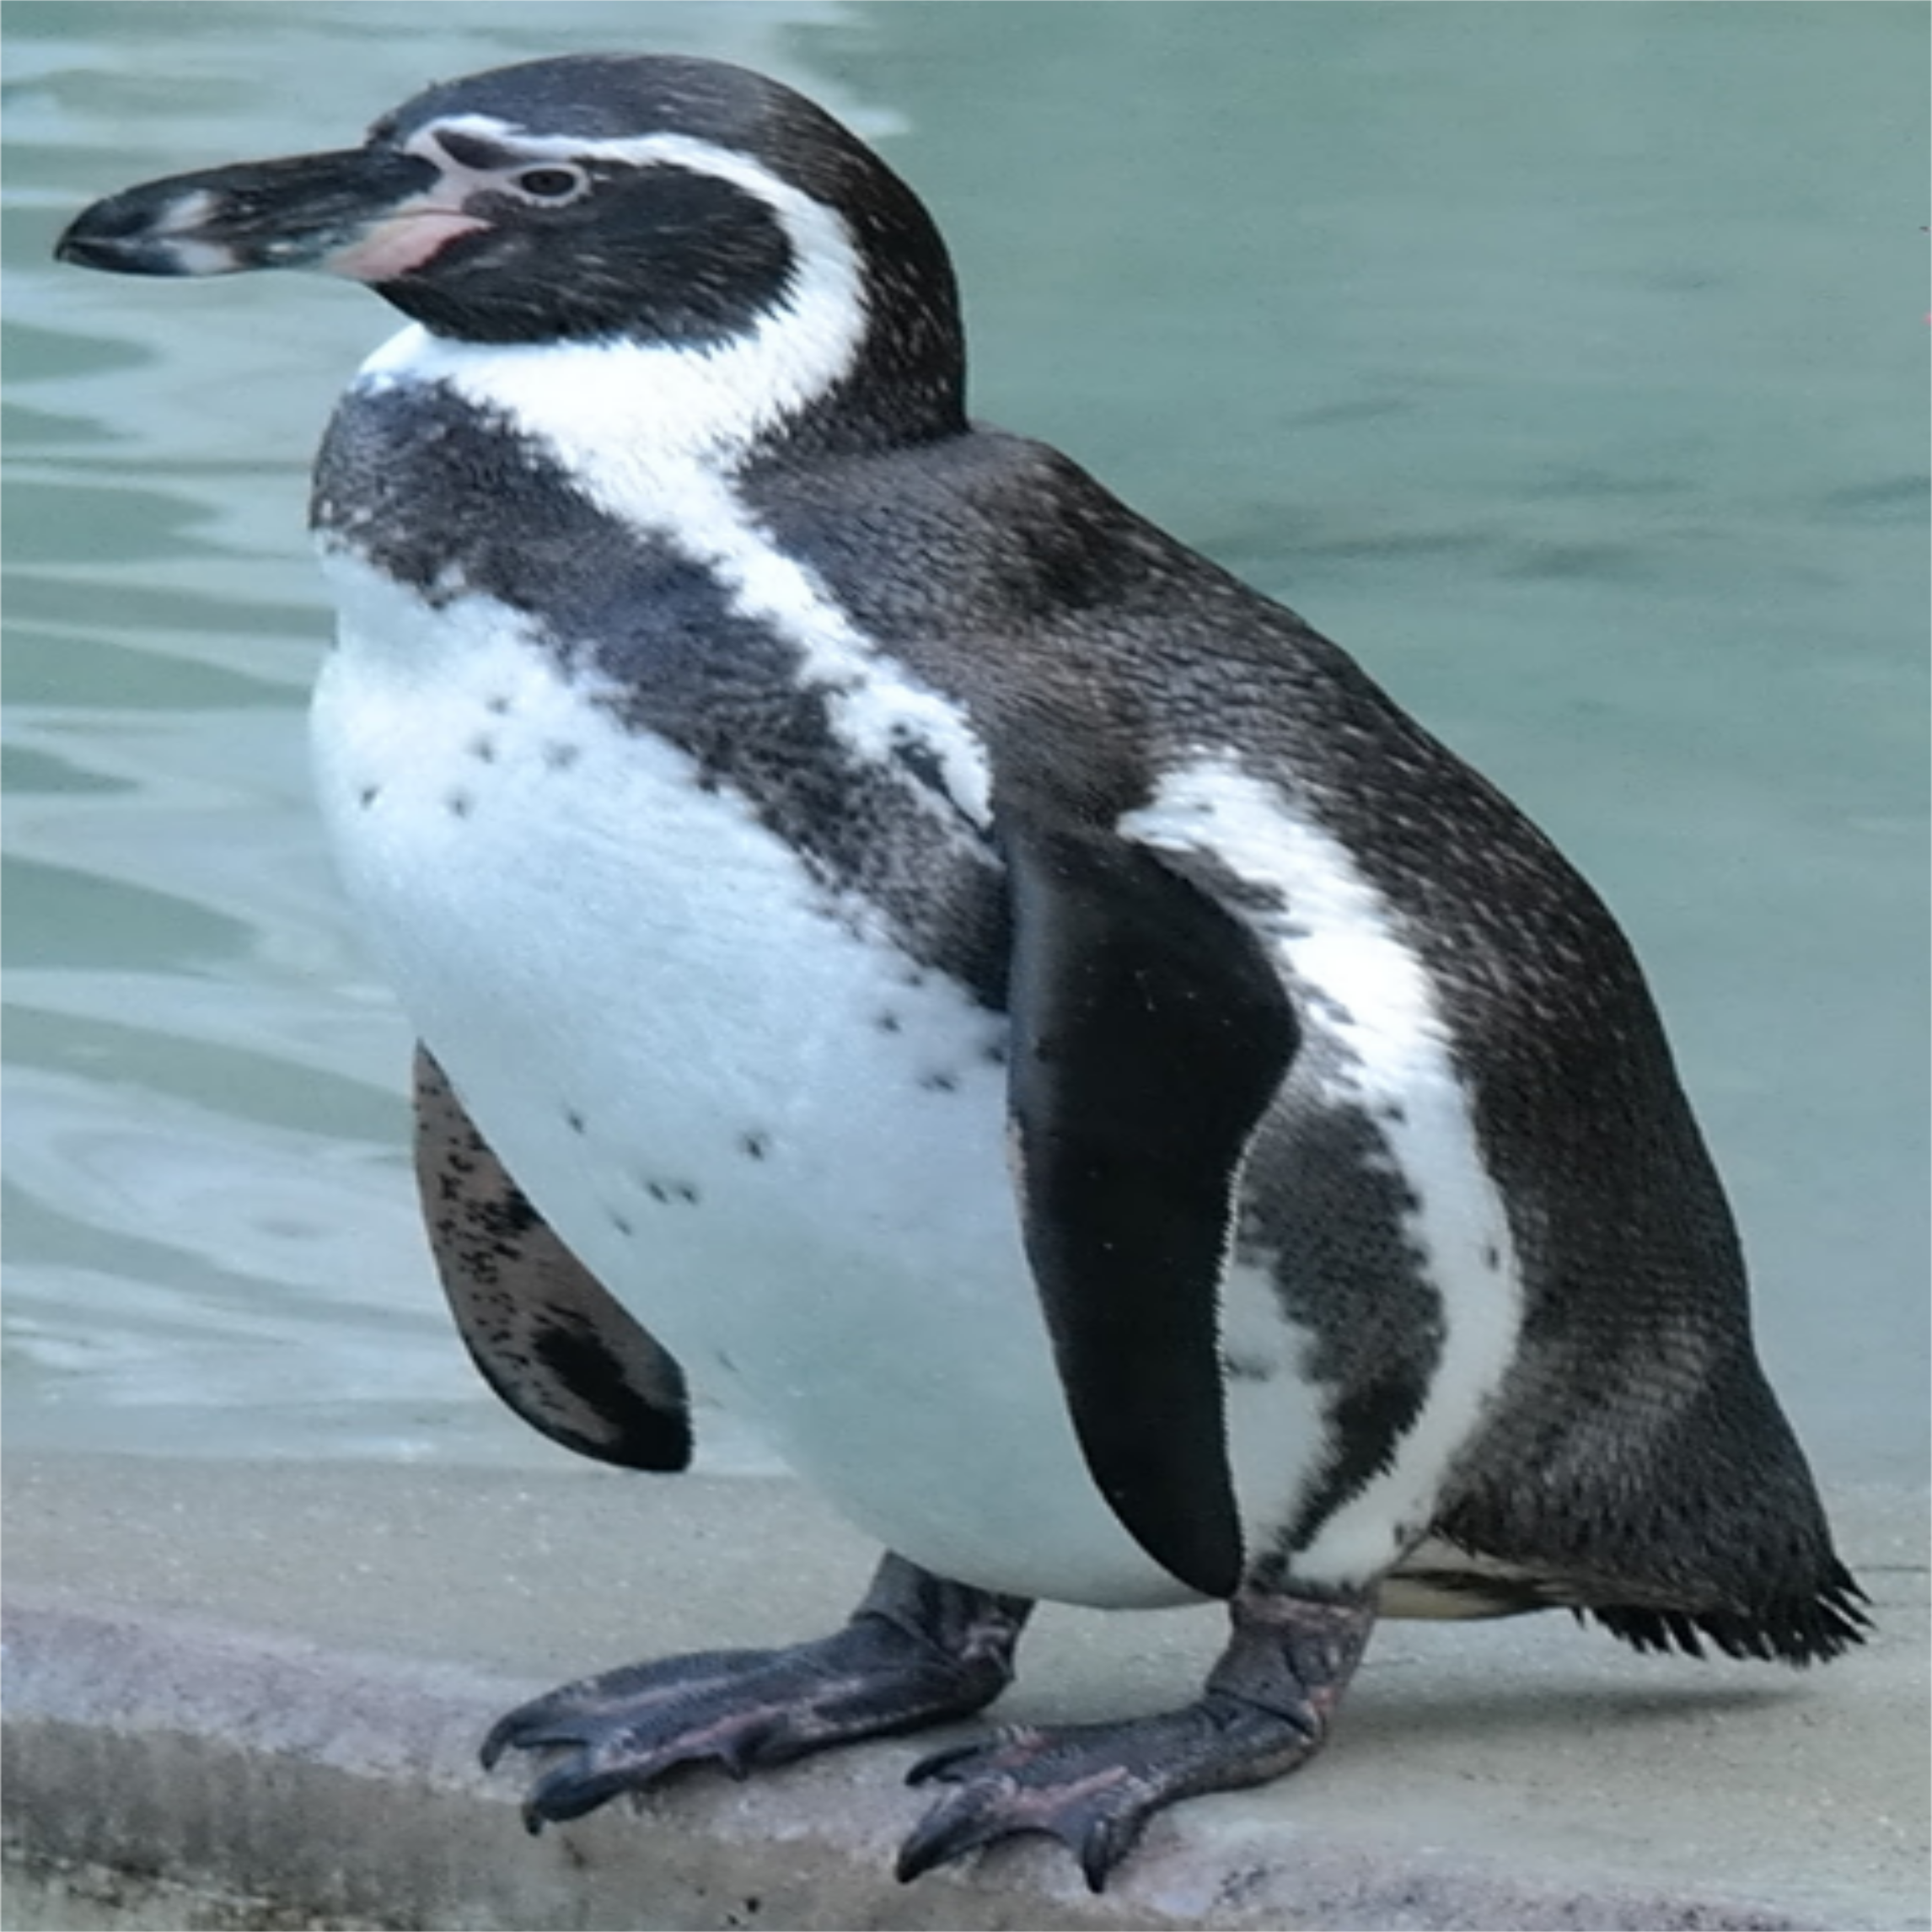
\includegraphics[height=4.2cm]{img/original-distortion.png}
         \caption{Rescaled}
     \end{subfigure}
     \hfill
     \begin{subfigure}[b]{0.3\textwidth}
         \centering
         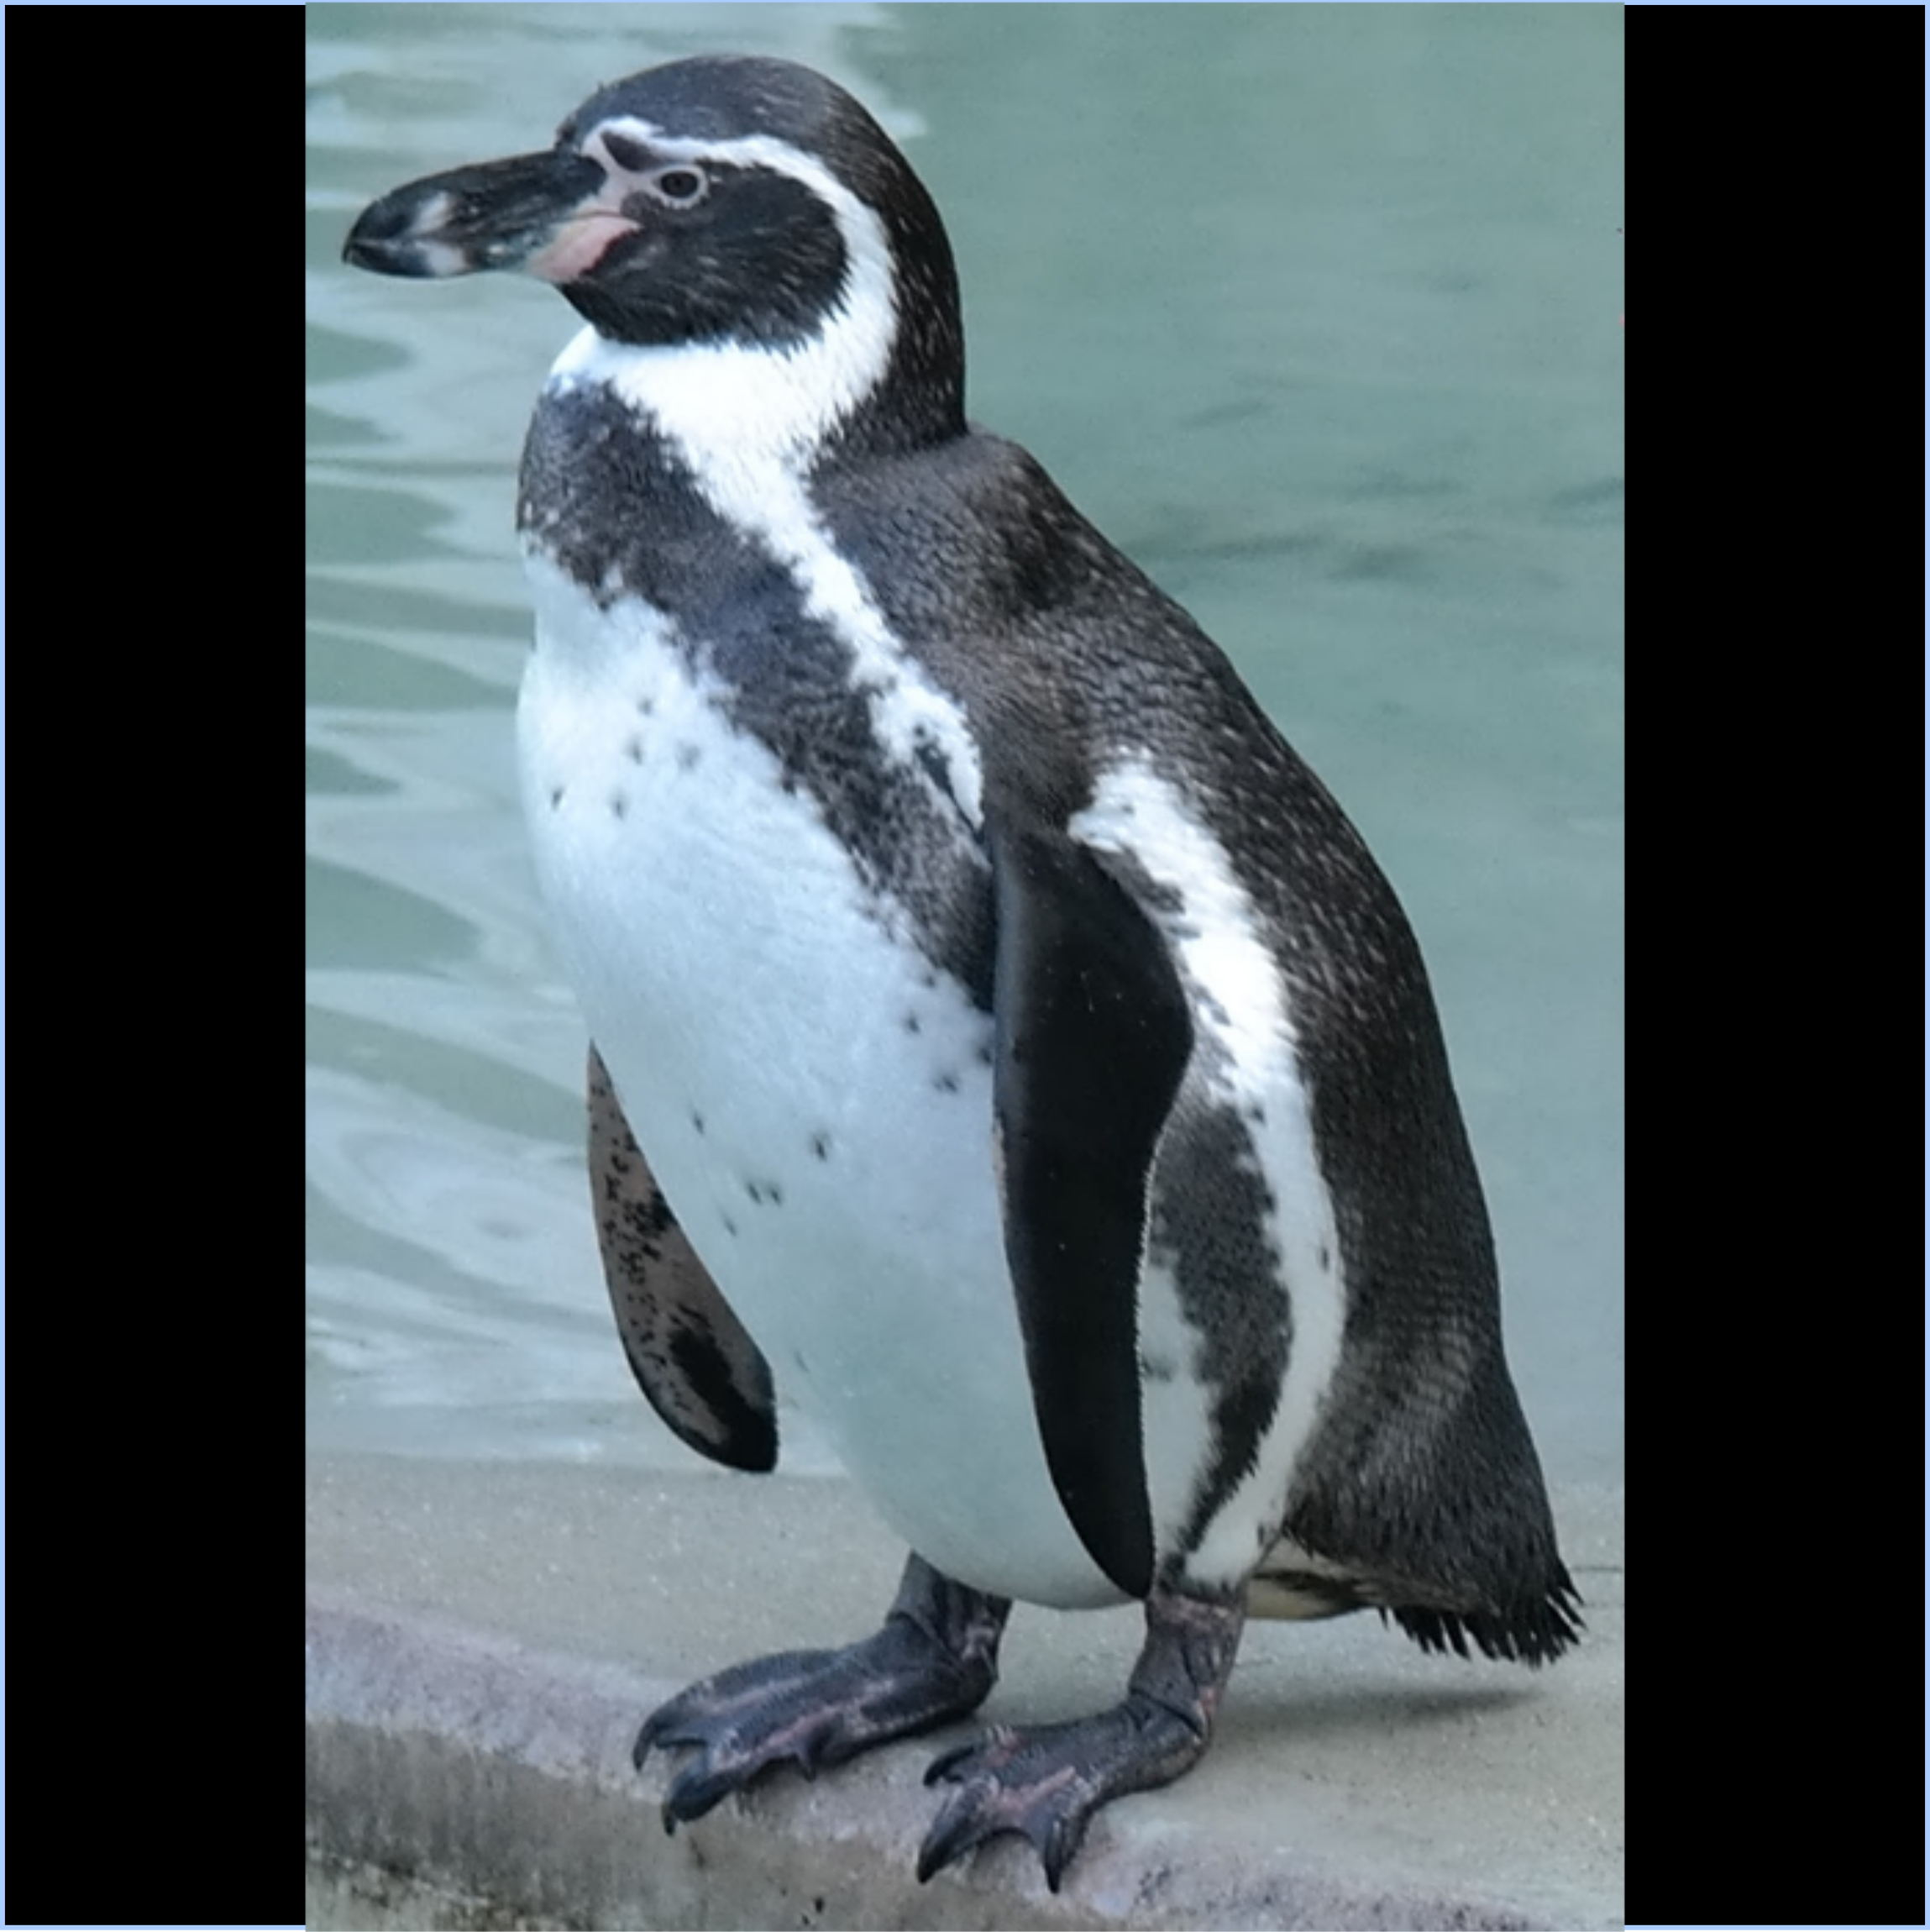
\includegraphics[height=4.2cm]{img/black_padding.png}
         \caption{Black padding}
     \end{subfigure}
        \caption{Overview of padding techniques}
        \label{fig:penguin}
\end{figure}

\subsection{Dimensionality reduction}

In this section, we take a look at reducing the dimensionality of the extracted features. Dimensionality reduction could help us to scale our approaches to even bigger datasets and to decrease the query response time.

The extracted features from the neural networks are from high-dimensional space (for MobileNetV2, it is 1280 features, for Resnet50 it is 2048 features). Moreover, the dimensionality reduction can also have a positive effect on reducing noise if present in the feature vector. We aim to evaluate the system with a reduced number of features. For the dimensionality reduction, we use the \acrlong{pca} (described in section \ref{s:pca}).

\subsection{Neural network selection}

At last, we discussed all the hyperparameters we aim to evaluate. In the evaluation sections, we run several experiments in order to find the best set of parameters. We use MobileNetV2 as our baseline feature extraction model due to its speed and small size.

After obtaining the best set of hyperparameters, we use the same set of hyperparameters for comparing the performance between different CNNs.

Aside from the MobileNetV2, we use two different instances of ResNet -- ResNet50 and ResNet50V2. Both ResNet50V2 and MobileNetV2 were trained on the classification task with 1000 classes. We include the ResNet50 as model pre-trained on more than eleven thousand classes\footnote{Source: \url{https://github.com/qubvel/classification\_models}}. We aim to experimentally support the claim that the network trained on more classes can achieve a better performance level. 

The downside of using ResNet50 trained on eleven thousands of classes compared to MobileNetV2 is slower evaluation and availability. Since the classification task on eleven thousand class is not one of the most common state-of-art challenges, the set of pre-trained neural network for this task is smaller. Also, used ResNet50 is only pre-trained with the input shape 224x224. To use it for the regions, we introduced upscaling for the network input. 

\chapter{Evaluations}
\label{ch:evaluation}

In this section, we provide evaluations for each aforementioned parameter of the framework. The presented evaluations are performed on the collected collages.

\section{Collected collages}

We manually created a set of queries to evaluate the proposed system's configurations. The figure \ref{fig:query_collage_comparison} shows one of such query -- target image and collage. The annotated data consists of 102 collages, each contains a visual description of a given target image. The average size of the images used in the collages covers 15\% of the canvas. Five percent of the collected collages contain an image bigger than 80\% of the canvas. We provide visualizations of the distribution of the annotated queries in figure \ref{fig:annotated_dataset}. We use total of 199 images to create these 102 collages.

\begin{figure}
     \centering
     \begin{subfigure}[b]{0.48\textwidth}
         \centering
         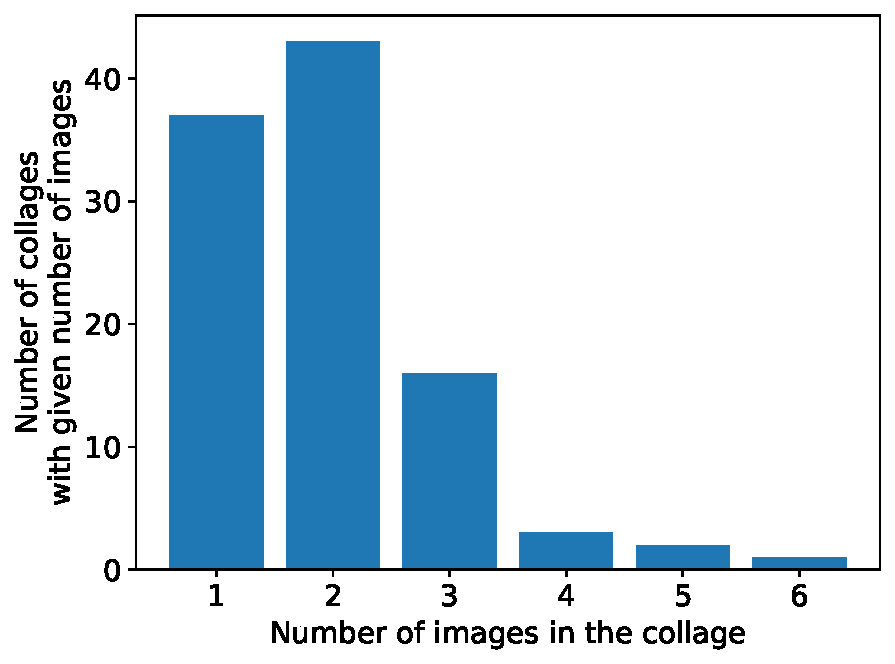
\includegraphics[width=\textwidth]{graphs/num_queries_in_request.pdf}
         \caption{Number of images on a canvas for a collage.}
     \end{subfigure}
     \hfill
     \begin{subfigure}[b]{0.48\textwidth}
         \centering
         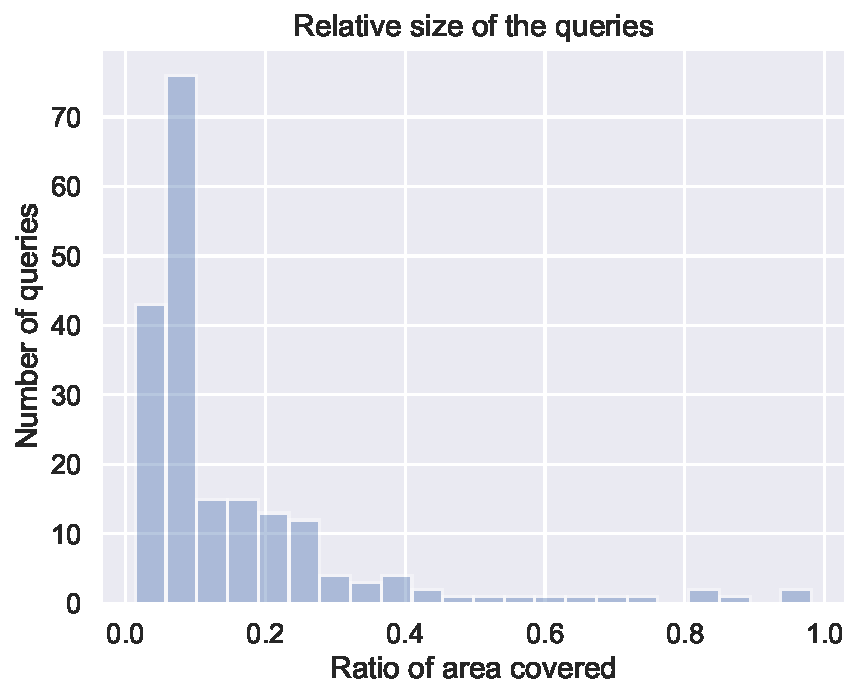
\includegraphics[width=\textwidth]{graphs/queries_size.pdf}
         \caption{Size of the canvas which is covered by a query image.}
     \end{subfigure}
    
    \caption{Collected collages properties}
    \label{fig:annotated_dataset}
\end{figure}

For the annotation, we used our application. It is possible to save the collage by clicking ``Submit Collage.'' The average time spent on creating a single collage was 91 seconds. This time includes searching for images online, pasting them onto the canvas, and also waiting for the responses of the system.

We want to highlight that we created more than a hundred collages corresponding to the target images from the dataset. The annotations were done only by a one person. We leave annotation from more people, to study the differences in behavior, for future work. 

\section{Plots overview}

Using the collected queries and based on the definition of the \emph{rank} we can visualize the performance of the system.

For this purpose we formulate a few additional terms. When measuring the performance system, we work on the set of collected queries $X$. For each of the query collage $Q_i$, we say that the rank of the target image $T_i$ is $r_D(T_i, Q_i)$ given the set of hyperparameters of the system $\theta$.

We define a function $s_{D, \theta, X}$, which represents the performance of the system.
$$
s_{D, \theta, X}:\{0, 1, \ldots |D| - 1\} \rightarrow \{0, 1, \ldots |X| - 1\}
$$  
$$
s_{D, \theta, X}(h) = \sum_{(T_i, Q_i) \in X}[r_D(T_i, Q_i) \leq h]
$$

In the plots we scale the both axis as the percentage of the dataset/collected queries. I.e., we display $r_D(T_i, Q_i) / |D|$ on $x$-axis and $s_{D, \theta, X}(h) / |X|$ on $y$-axis. That way we obtain comparable results even in case of different datasets. 

Similarly to our reasoning in section \ref{s:task_formulation} we claim that this function correlates with the time spent on retrieving all target images.


\section{Summary}

In this chapter, we focus on fine-tuning several hyperparameters of the task at hand. We achieved the best results using the approach of cutting the image into regions, with settings of 2x4 and 3x5 regions. Additionally, we showed that the best performing input shapes were $96\times 96$ and $128 \times 128$.  We did not found out that the number of selected crops would play a significant role in the performance of tested variants. For the distance function, we chose \emph{cosine distance} since it performed significantly better than the other evaluated distance functions. To aggregate the distances, we selected the averaging function as it led to the best results. For the padding selection, it emerged from the experiment that \emph{rescale} worked the best. From the tested networks, \emph{Resnet50} trained on eleven thousands of classes performed the best. Finally, we concluded that dimensionality reduction into \emph{128} dimensions have a little, almost no negative effect on the performance of the system. Therefore we recommend using it. 



\begin{figure}
    \centering
    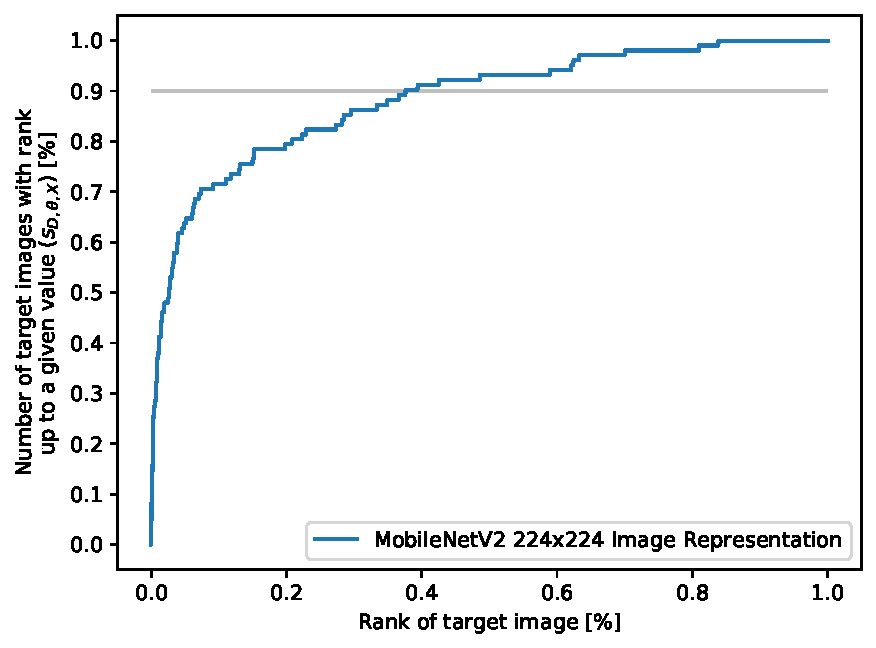
\includegraphics[width=0.8\linewidth]{graphs/dd20090d2f746141e927422ef0528eed6141a2d1478d86afe3d450e0c99e9765.pdf}
    \caption{Performance of MobileNetV2 in the Baseline -- Image representation setting}
    \label{fig:mobilenet_whole_image_example}
\end{figure}

\begin{figure}
\centering
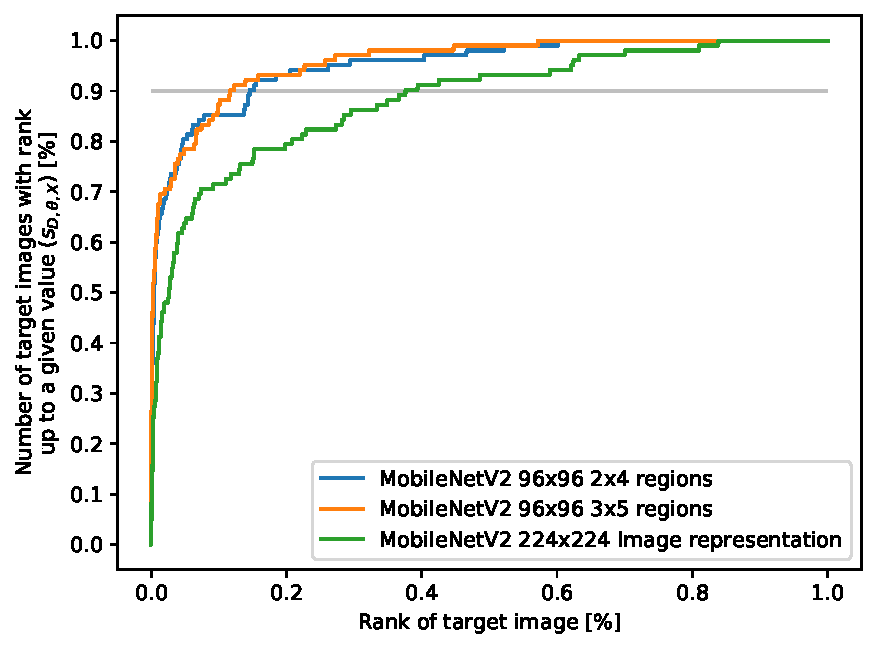
\includegraphics[width=0.8\linewidth]{graphs/0c36458e4a7754f349e4dd02e823acc5f192f0aaa42647313045530525f3db19.pdf}
\caption{An experiment comparing the effect of the changing number of regions.}
\label{fig:different_number_regions}
\end{figure}

\begin{figure}
\centering
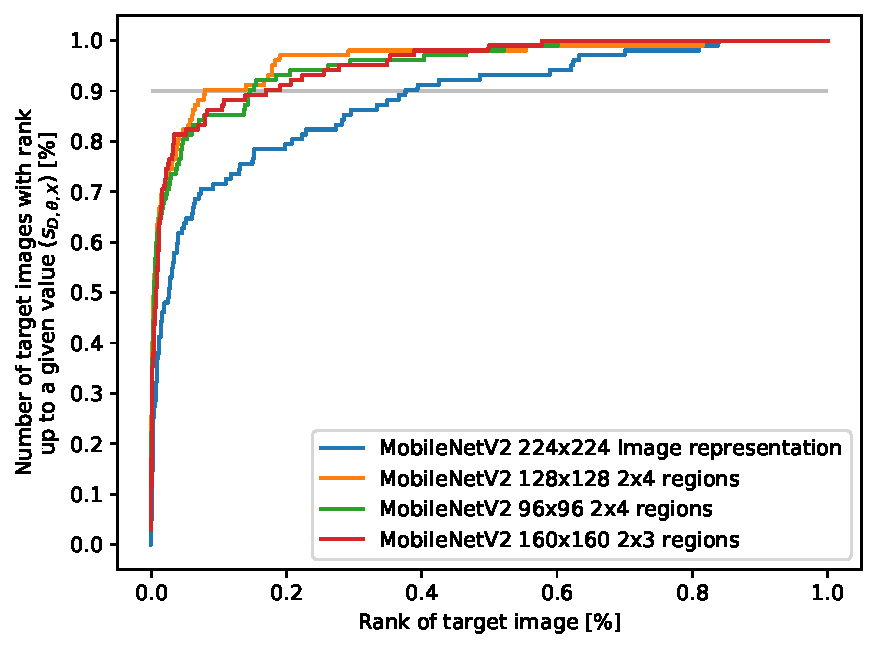
\includegraphics[width=0.8\linewidth]{graphs/901175c0015f71987720d10953133afa566d88a09a6d7182a074859ff4e8409e.pdf}
\caption{An experiment comparing the effect of the changing regions size.}
\label{fig:different_region_size}
\end{figure}

\begin{figure}
\centering
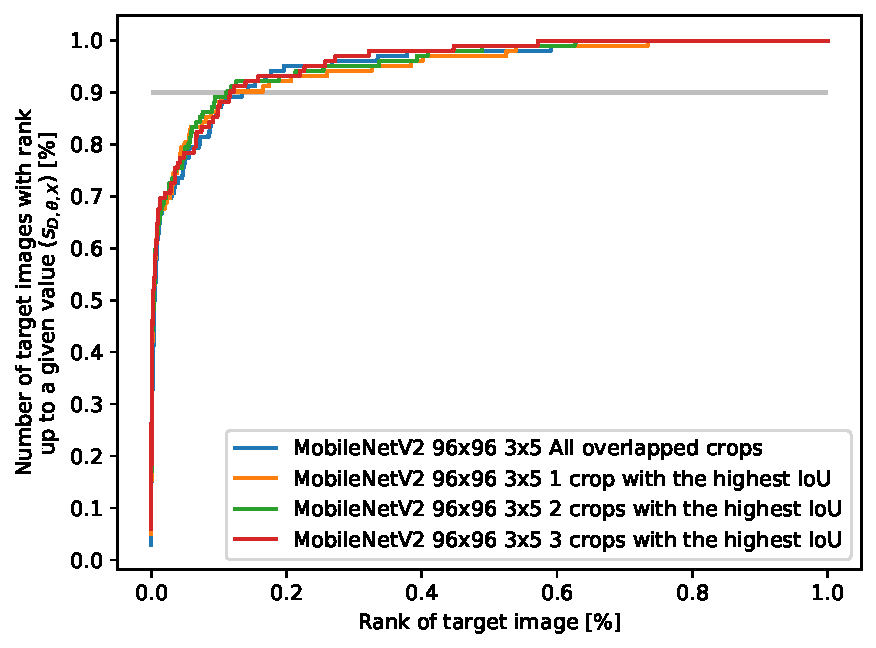
\includegraphics[width=0.8\linewidth]{graphs/5c4a781f8e6f3eac93db2083bde3963c06582a92a8141411bf29e41251a98e75.pdf}
\caption[Performance of the system based on different number of chosen crops]{Performance of the system based on different number of chosen crops. This experiment shows only a minor change in performance with the increasing number of selected regions.}
\label{fig:crop_limitation}
\end{figure}

\begin{figure}
    \centering
    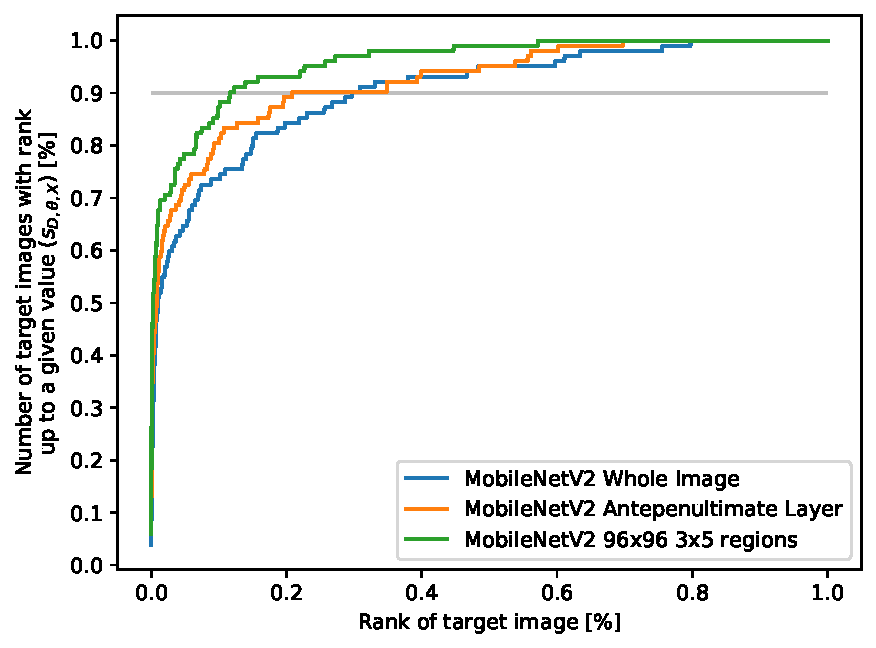
\includegraphics[width=0.8\linewidth]{graphs/adaf8d435bb40406f9ce40654ec396e04453ab76cf0776d2a87d385055d5424f.pdf}
    \caption[Comparison of baseline, regions and approach using the output of the layer before the global pooling]{Comparison of baseline, regions and approach using the output of the layer before the global pooling. Due to higher memory requirements, we had to sample the dataset. We randomly sampled one-tenth of the dataset. We also provide a baseline on this smaller dataset, the performance may slightly change, based on the dataset. We can see that using the information from the layer, before the global pooling layer improved the performance of the system, compared to the baseline. These are interesting results, because, that the underlying network is for both approaches identical. This shows, that we can elevate the spatial information about the objects from the last convolution block.}
    \label{fig:antepenultimate}
\end{figure}

\begin{figure}
    \centering
    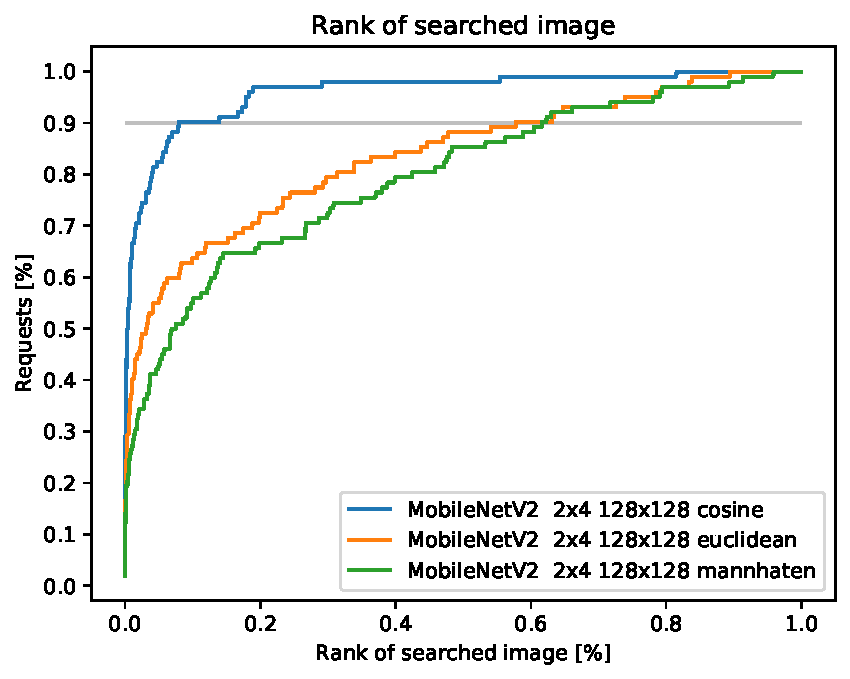
\includegraphics[width=0.8\linewidth]{graphs/3aab502ea602a9f49afaa0a0d998cf226a0a67b9efcaa655d2ddf5063eeabe47.pdf}
    \caption{Comparison of the performance based on the chosen distance function. We see a superior performance of the cosine distance.}
    \label{fig:regions_distances}
\end{figure}

\begin{figure}
\centering
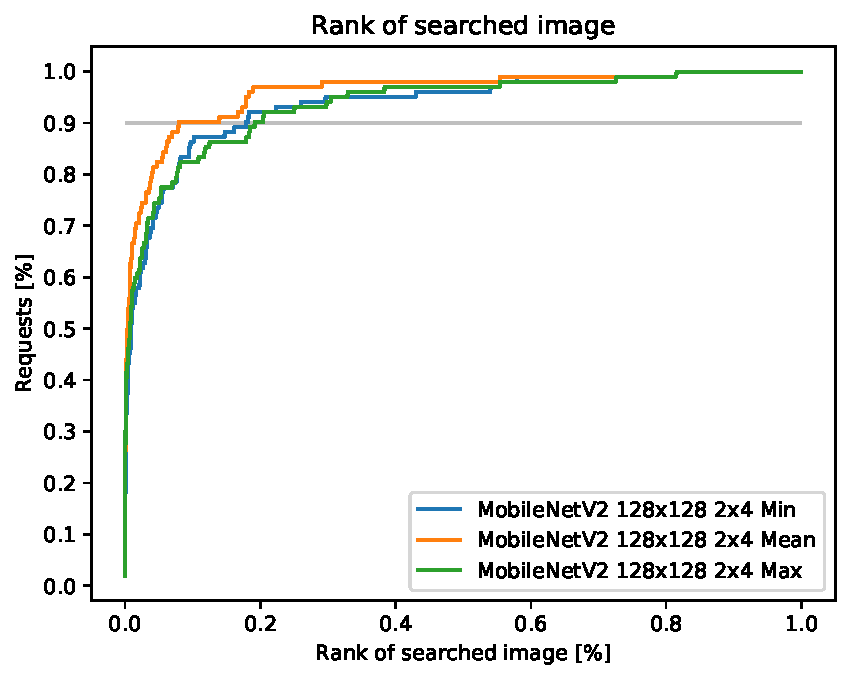
\includegraphics[width=0.8\linewidth]{graphs/70c56dc52be92e048f57b9bdfb35ddce2be41fd2454ae360588da2e387b09de5.pdf}
\caption{Performance of the system based on different aggregation function}
\label{fig:ranking_funcs}
\end{figure}

\begin{figure}
    \centering
    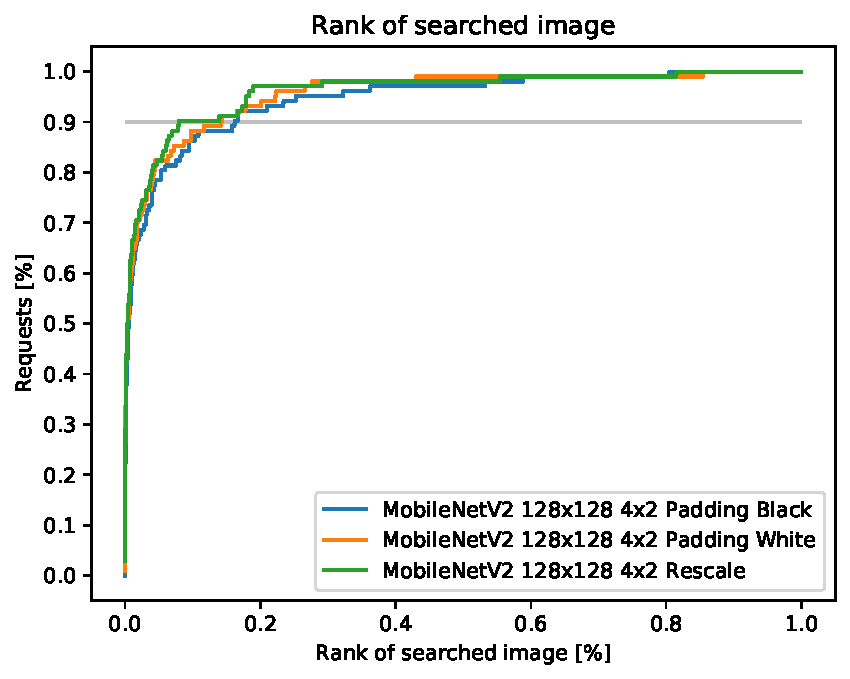
\includegraphics[width=0.8\linewidth]{graphs/bf57efafbbbc7b5a1744054d87d4ecfa381c9eaf2459186904190d97bcb99a81.pdf}
    \caption[Comparison of different padding method for images in the query]{Comparison of different padding method for images in the query. Based on the experiment, rescaling is the best option.}
    \label{fig:padding}
\end{figure}

\begin{figure}
    \centering
    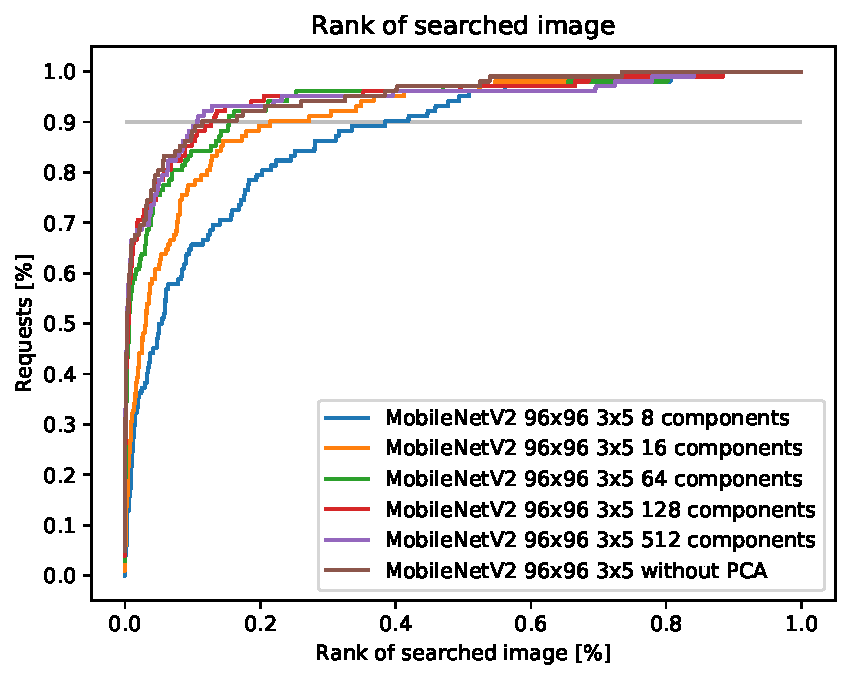
\includegraphics[width=0.8\linewidth]{graphs/6fbd4f70810e1f63f400ef601c1cdba0fd1635749810aa2347a4ff26e6fccf47.pdf}
    \caption[Effect of \acrshort{pca} on the performance of the system]{Effect of \acrshort{pca} on the performance of the system. The results offer several interesting observations. With the increasing number of components, the system performs better. With 512 components, it even performed slightly better than on the original data. For our purposes, we conclude that selecting 128 components offer the best performance-cost ratio. With the need for smaller feature vectors, we would select at minimum 64 components.}
    \label{fig:pca}
\end{figure}

\begin{figure}
    \centering
    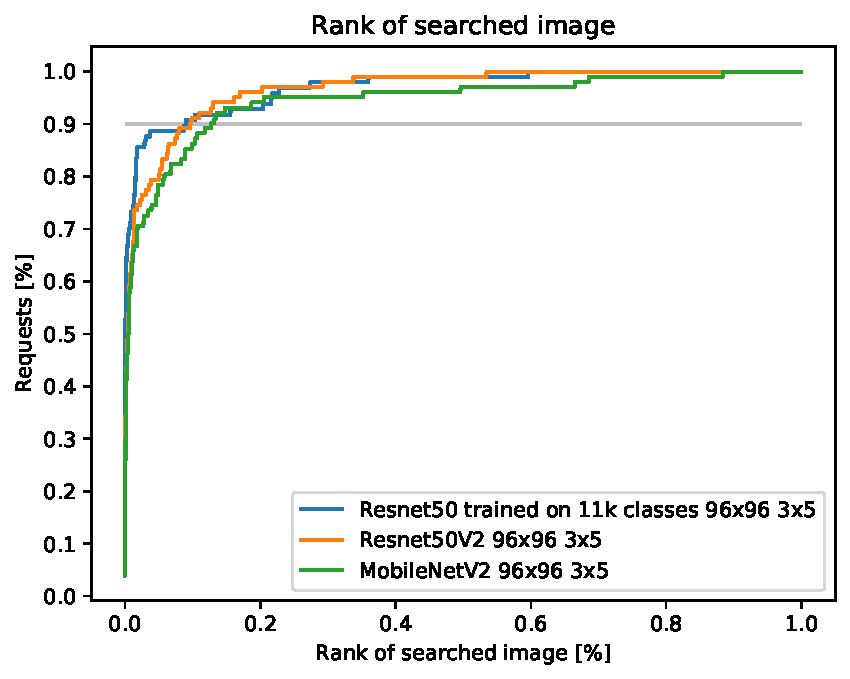
\includegraphics[width=0.8\linewidth]{graphs/2536f6c96149dea24dae84dbf52f760d7d58b0dffa7d660656e1784d9dca277f.pdf}
    \caption[Comparison of the performance based on different feature extraction models]{Comparison of the performance based on different feature extraction models. The performance of the Resnet50 trained on 11 thousands of classes is better compared to the other two. This experiment shows results after performing the \acrshort{pca} to 128 dimensions.}
    \label{fig:networks}
\end{figure}
